\documentclass{article}

\usepackage{ctex}
\usepackage[left=1.25in,right=1.25in,top=1in,bottom=1in]{geometry}
\usepackage{amsmath}
\usepackage{amssymb}
\usepackage{graphicx}
\usepackage{float}
\usepackage{subfigure}
\usepackage{listings}
\usepackage{xcolor}
\lstset{language=Python}   
\lstset{breaklines}              
\lstset{extendedchars=false}
\lstset{ 
	backgroundcolor=\color{white},   % 选择代码背景,必须加上\ usepackage {color}或\ usepackage {xcolor}.
	basicstyle=\footnotesize,        % 设置代码字号.
	breakatwhitespace=false,         % 设置是否当且仅当在空白处自动中断.
	breaklines=true,                 % 设置自动断行.
	captionpos=b,                    % 设置标题位置.
	commentstyle=\color{mygreen},    % 设置注释格式
	deletekeywords={...},            % 是否删除给定语言的关键词.
	escapeinside={\%*}{*)},          % 是否在代码中添加LaTex.
	extendedchars=true,              % 是否允许使用非ASCII字符; 仅适用于8位编码,不适用于UTF-8. 
	frame=single,	                   % 给代码区添加边框.
	keepspaces=true,                 % 保留空格(useful for keeping indentation of code (possibly needs columns=flexible).
	keywordstyle=\color{blue},       % 关键字显示风格.
	language=Octave,                 % 使用的语言.
	morekeywords={*,...},            % 是否需要添加其他的关键词.
	numbers=left,                    % 给代码添加行号,可取值none, left, right.
	numbersep=5pt,                   % 设置行号与代码之间的间隔
	numberstyle=\tiny\color{mygray}, % 行号的字号和颜色
	rulecolor=\color{black},         % 边框颜色,如果没有设置,框架颜色可以在非黑色文本中的换行符上更改(例如 text (e.g. comments (green here)))
	showspaces=false,                % 显示每个地方添加特定下划线的空格; 覆盖了'showtringspaces'
	showstringspaces=false,          % 仅在字符串中允许空格
	showtabs=false,                  % show tabs within strings adding particular underscores
	stepnumber=2,                    % the step between two line-numbers. If it's 1, each line will be numbered
	stringstyle=\color{mymauve},     % string literal style
	tabsize=2,	                   % 将默认tab设置为2个空格
	title=\lstname                   % show the filename of files included with \lstinputlisting; also try caption instead of title
}

\usepackage[framed,numbered,autolinebreaks,useliterate]{mcode}

\author{张泽宇}
\date{2022年5月8日}
\title{第十、十一周工作总结}

\begin{document}
	\maketitle
	
	{\centering \rule[15pt]{15cm}{0.1em}}
	
	{
		\noindent
		\large
		\textbf{过去两周的主要进行的工作包括有:
			\begin{itemize}
				\item 修改原来的仿真模型,调整了故障持续时间,添加过渡电阻。
				\item 就改进后的模型调整了灰度图的生成方式,并将三相电流都作为输入生成灰度图,得到了较好的效果。
				\item 学习了PyTorch框架,基于PyTorch搭建神经网络模型,模型结构参考LeNet-5进行构建,对灰度图进行训练学习,得到较好的结果。
				\item 学习了TensorBoard的使用,可视化了神经网络结构和训练过程。
			\end{itemize}
	}}
	
	以下为详细叙述
	
	{\centering \rule[-10pt]{15cm}{0.1em}}
	
	\newpage
	
	\section{仿真模型的修改}
	
	针对上周出现的问题,李教授给出了非常有用的建议。模型的改进主要体现在如下两点。
	
	\subsection{故障时间调整}
	
	首先回归最简单的情况,不考虑故障发生时间的延迟和故障位置,只考虑故障发生的类型,简化问题。考虑到初始状态下电源电压为0,有一个短暂的建立稳态的过程,因此假设故障在0.04s发生,持续到仿真结束,即永久性故障。从定性的角度来讲,这样更为合理的原因可能在于取多个故障周期,可以收集更多的故障特征,反应在灰度图上,即为不同故障类型的图像特征更为明显,可以避免上次多种情况下灰度图都只是一条黑纹的情况。
	
	当永久性故障可以得到较好的目标效果后,再进一步考虑故障结束和故障发生时间延迟,最后考虑不同的故障发生地点。
	
	\subsection{过渡电阻设置}
	
	在故障发生点增加一个1000$\Omega$的电阻。这样的目的是为了控制短路时故障电流不至于太大,同时将电路中的每个负载增大,使正常运行时存在一定的电流。这样可以避免上一周中故障电流与正常电流之间数量级差别太大。
	
	这里选择1000$\Omega$是基于试验的结果,当过渡电阻为这个值时,故障电流和故障电压之间的数量级控制在$10^{1}$之内。理论来讲,过渡电阻的阻值应当依据具体电路而定,没有固定值。
	
	基于上面两种改进,得到了仿真模型的控制部分如下图所示:
	
	\begin{figure}[h]
		\centering
		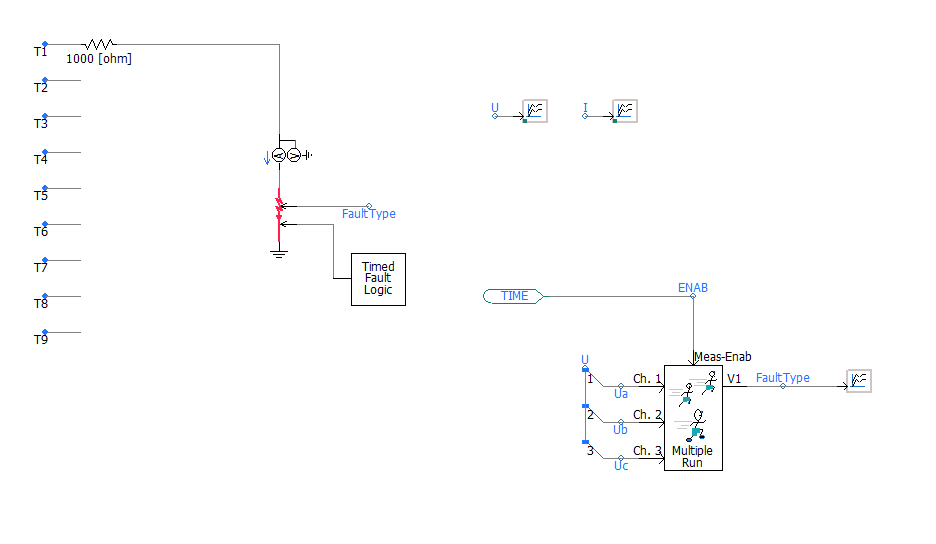
\includegraphics[width=13cm]{figure/1.png}
		\caption{改进后的模型控制部分}
	\end{figure}
	
	\section{调整灰度图的生成方式}
	
	主要修改了两个部分:
	
	\subsection{将三相电流整合}
	
	听取李教授的建议,将三相电流全部作为输入生成灰度图。经过思考,我认为这样做是非常必要的。例如,如果只是单将一相电流作为输入,在三相对称的前提下,由于A、B、C单相短路接地时故障电流电压在时域上波形特征相同,只是发生时间推迟一些,在加上故障延迟的条件,很容易出现特征相似的情况。而如果将三相电流都作为输入,就可以避免这种情况,提高数据集的质量。
	
	同时,三相电流必须以($i_{A}\mid_{t=t1}$、$i_{B}\mid_{t=t1}$、$i_{C}\mid_{t=t1}$、$i_{A}\mid_{t=t2}$、$i_{B}\mid_{t=t2}$、$i_{C}\mid_{t=t2}$ \dots )的形式进行组织。因此添加了Mix\_data函数,用Flatten的F模式合并读取到的数据。
	
	\begin{lstlisting}
	def Mix_data(data):
		dic = {'FaultType': data['FaultType']}
		temp_U = np.array((data['U_1'], data['U_2'], data['U_3']))
		dic['U'] = temp_U.flatten('F')
		temp_I = np.array((data['I_1'], data['I_2'], data['I_3']))
		dic['I'] = temp_I.flatten('F')
		return dic
	\end{lstlisting}

	\subsection{调整了灰度图像的大小}
	
	这部分改进是基于每次仿真时间为0.2s,channel输出步长为10$\mu s$,因此可以得到20000个数据点。对此,采用128$\times$128=16384的灰度图更为合适。而且由于0.04s开始发生故障,因此随机截取的灰度矩阵中可以包含故障发生的大部分数据和故障前的小部分数据。
	
	基于上述两处改动,并对程序的一些细节部分进行优化,得到了最终的灰度图像,如图3至图6所示:
	
	\begin{figure}[ht]
		\centering
		\subfigure{
			\begin{minipage}[t]{0.4\linewidth}
				\centering
				
\includegraphics[width=2in]{figure/2.jpg}
				\caption{A相短路接地}
			\end{minipage}
		}
		\subfigure{
			\begin{minipage}[t]{0.4\linewidth}
				\centering
				
\includegraphics[width=2in]{figure/3.jpg}
				\caption{AB相短路接地}
			\end{minipage}
		}
		
		\subfigure{
			\begin{minipage}[t]{0.4\linewidth}
				\centering
				
\includegraphics[width=2in]{figure/4.jpg}
				\caption{ABC三相短路接地}
			\end{minipage}
		}
		\subfigure{
			\begin{minipage}[t]{0.4\linewidth}
				\centering
				
\includegraphics[width=2in]{figure/5.jpg}
				\caption{AB相短路}
			\end{minipage}
		}
		
	\end{figure}

	可以看出,相比于上周的结果,灰度图之间有较为明显的差异性。每种故障先生成500张灰度图,得到共2000张灰度图的数据集。
	
	\section{基于PyTorch的神经网络搭建}
	
	之所以转用PyTorch平台,是因为在之间的学习中,我发现Matlab构建神经网络太考验计算机性能,Matlab对计算机内存要求有点高,这个和它的程序工作原理有一些关系,导致一些改动和想法都无法实现,同时每次神经网络的训练经历的时间比较长,所以用三周左右的时间学习了PyTorch框架,利用PyThon进行深度学习更容易实现,同时对模型的计算转到GPU上运行,计算速度得到了极大的提升。现将整个过程复述如下:
	
	\subsection{神经网络搭建}
	
	利用PyTorch的现有函数,可以快速搭建神经网络。这部分程序如下:
	
	\begin{lstlisting}
	import torch
	from torch import nn
	from torch.utils.tensorboard import SummaryWriter
		
		
	class Net(nn.Module):
		def __init__(self):
			super(Net, self).__init__()
			self.module = nn.Sequential(
			nn.Conv2d(in_channels=1, out_channels=16, kernel_size=(5, 5)),
			nn.ReLU(),
			nn.MaxPool2d(kernel_size=(8, 8)),
		
			nn.Conv2d(in_channels=16, out_channels=32, kernel_size=(5, 5)),
			nn.ReLU(),
			nn.MaxPool2d(kernel_size=(2, 2)),
		
			nn.Flatten(),
		
			nn.Linear(in_features=32*5*5, out_features=256),
			nn.Linear(in_features=256, out_features=36),
			nn.Linear(in_features=36, out_features=4)
			)
		
		def forward(self, x):
			x = self.module(x)
			return x
		
		
	if __name__ == '__main__':
		net = Net()
		input = torch.ones((32, 1, 128, 128))
		output = net(input)
		print(output.shape)
		writer = SummaryWriter('log_net')
		writer.add_graph(net, input)
		writer.close()
	\end{lstlisting}
	
	需要指明,这次的神经网络是在现有的LeNet-5模型上搭建的,与以往自己的模型不同。LeNet-5模型是一个CNN的经典结构\footnote{http://yann.lecun.com/exdb/lenet/index.html},主要是用于手写字体的识别。它的输入为32像素图像,用来进行10分类。由于LeNet-5模型较为简易而且在简单图像识别上表现较优,所以借鉴其结构。但是由于输入、输出都不相同,所以在结构的基础上对参数进行修改。
	
	在代码中,使用TensorBoard记录模型的信号流向,但是Flow图对网络结构表现得不是很清晰,所以又使用一种工具绘制了模型的结构,如下图6所示(由于svg图像无法在latex中引入,转成png图像时有一定的矢量损失,所以图像变模糊,后期探索有无解决方法):
	
	\begin{figure}[h]
		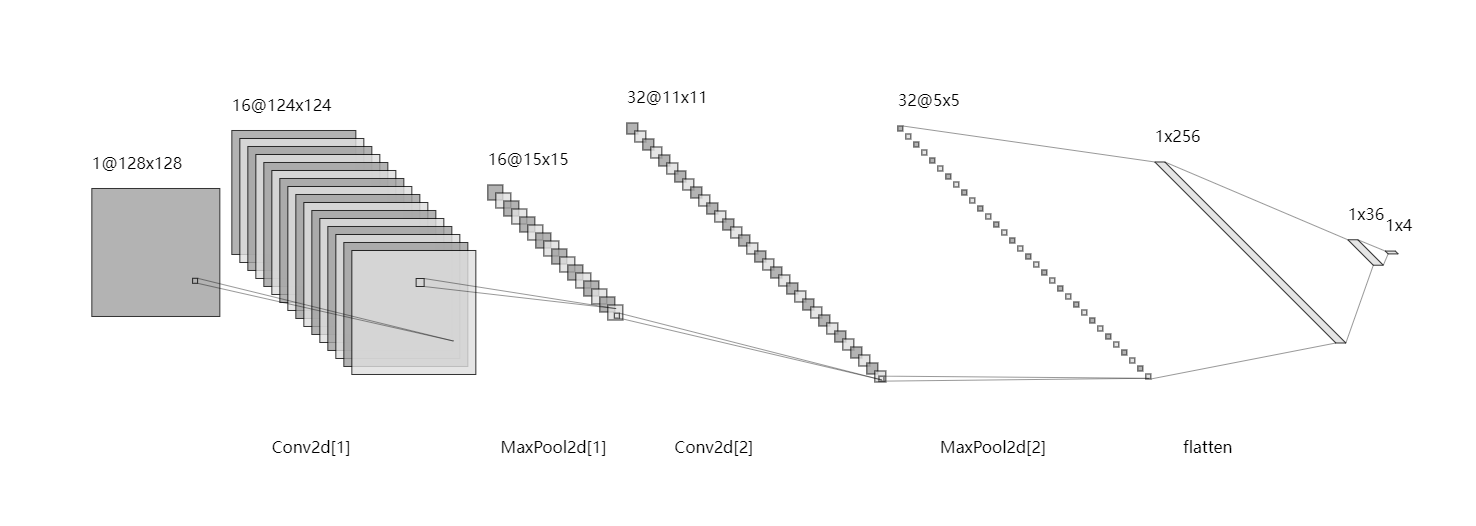
\includegraphics[width=15cm]{figure/6.png}
		\caption{模型结构}
	\end{figure}

	直观来讲,网络在第一层池化时kernel\_size参数设置有些过大,可以进行优化。
	
	\subsection{数据集准备}
	
	采用PyTorch提供的Dataset类制作数据集,格式为文件夹名为标签名,这里用1、4、7、8代表单相短路接地、两相短路接地、三相短路接地、两相短路。将总体数据随机选择10\%作为验证集。这部分代码如下:
	
	\begin{lstlisting}
	import torch
	from torch.utils.data import Dataset, random_split
	import os
	from PIL import Image
	from torchvision import transforms
		
		
	class ReadData(Dataset):
		def __init__(self, root_dir, label_dir):
			self.root_dir = root_dir
			self.label_dir = label_dir
			self.path = os.path.join(self.root_dir, self.label_dir)
			self.img_path = os.listdir(self.path)
			self.transforms = transforms.ToTensor()
		
		def __getitem__(self, idx):
			img_name = self.img_path[idx]
			img_item_path = os.path.join(self.root_dir, self.label_dir, img_name)
			img = Image.open(img_item_path)
			img = self.transforms(img)
			label = eval(self.label_dir) 
			if label == 1:
				label = 0
			elif label == 4:
				label = 1
			elif label == 7:
				label = 2
			elif label == 8:
				label = 3
			else:
				label = 'wrong'
			label = torch.tensor(label)
			return img, label
		
		def __len__(self):
			return len(self.img_path)
		
		
		data_dir = ''
		type1_label_dir = '1'
		type2_label_dir = '4'
		type3_label_dir = '7'
		type4_label_dir = '8'
		
		type1_dataset = ReadData(data_dir, type1_label_dir)
		type2_dataset = ReadData(data_dir, type2_label_dir)
		type3_dataset = ReadData(data_dir, type3_label_dir)
		type4_dataset = ReadData(data_dir, type4_label_dir)
		
		len_train = 450
		len_test = 50
		train_type1_dataset, test_type1_dataset = random_split(
		dataset=type1_dataset,
		lengths=[len_train, len_test],
		generator=torch.Generator().manual_seed(0)
		)
		train_type2_dataset, test_type2_dataset = random_split(
		dataset=type2_dataset,
		lengths=[len_train, len_test],
		generator=torch.Generator().manual_seed(0)
		)
		train_type3_dataset, test_type3_dataset = random_split(
		dataset=type3_dataset,
		lengths=[len_train, len_test],
		generator=torch.Generator().manual_seed(0)
		)
		train_type4_dataset, test_type4_dataset = random_split(
		dataset=type4_dataset,
		lengths=[len_train, len_test],
		generator=torch.Generator().manual_seed(0)
		)
		
		train_dataset = train_type1_dataset + train_type2_dataset + train_type3_dataset + train_type4_dataset
		test_dataset = test_type1_dataset + test_type2_dataset + test_type3_dataset + test_type4_dataset
	\end{lstlisting}
	
	在这个程序中,打标签的过程(22至32行)存在一些需要优化的地方。因为Tensor没有字符串的变量类型,针对这个问题可以把1、4、7、8由str类转为int类参与后面的运算,但是如果故障类型增加,由于损失函数计算是按照预测输出序列最大值的索引进行,那么第五类故障的索引4就会和标签4冲突,导致计算产生问题。所以这里选择把1、4、7、8重新打上1、2、3、4的标签,既不影响损失的计算,也可以避免发生冲突。但这并不是一个常用普遍的方法。
	
	\subsection{训练过程}
	
	训练过程分为:数据集导入、设置训练参数、设置训练、设置验证、数据记录五个模块。
	
	\subsubsection{数据集导入}
	
	\begin{lstlisting}
	train_data_set = Readdata_V2.train_dataset
	test_data_set = Readdata_V2.test_dataset
	
	train_data_size = len(train_data_set)
	test_data_size = len(test_data_set)
	
	print('========================================')
	print('训练集的长度为:{}'.format(train_data_size))
	print('测试集的长度为:{}'.format(test_data_size))
	print('========================================')
	
	train_data_loader = DataLoader(train_data_set, batch_size=1, shuffle=True)
	test_data_loader = DataLoader(test_data_set, batch_size=1, shuffle=True)
	\end{lstlisting}

	这部分代码中有一个很关键的参数,shuffle=True,因为在数据集的制作过程中,(上个代码的73、74行)只是将不同故障类别的灰度图叠加,没有做打乱顺序处理,因此在数据排布上是按照四种故障依次出现的顺序。如果shuffle设置为False,每批次取出图片前不打乱顺序,就会导致模型先对1故障训练,再对4故障训练,以此类推,最后的损失函数波动较大,虽然也能收敛,但是训练过程不很完善。
	
	\subsubsection{设置训练参数}
	
	\begin{lstlisting}
	learning_rate = 0.01
	epochs = 10
	total_train_step = 0
	total_test_step = 0
	
	net = Net_V2.Net()
	net.cuda()
	
	loss_fc = nn.CrossEntropyLoss()
	loss_fc.cuda()
	optimizer = torch.optim.SGD(params=net.parameters(), lr=learning_rate)
	writer = SummaryWriter('logs')
	\end{lstlisting}

	学习率取0.01,训练10轮,损失函数采用交叉熵损失函数,优化方法选用随机梯度下降法,并利用Tensorboard记录训练过程。同时把网络和损失的计算放在GPU上进行,提升运算速率。
	
	\subsubsection{设置训练和验证}
	
	\begin{lstlisting}
	for epoch in range(epochs):
		print("-------第{}轮训练开始--------".format(epoch + 1))
		
		for data in train_data_loader:
			imgs, labels = data
			imgs = imgs.cuda()
			labels = labels.cuda()
			outs = net(imgs)
			loss = loss_fc(outs, labels)
		
			optimizer.zero_grad()
			loss.backward()
			optimizer.step()
			total_train_step += 1
			writer.add_scalar('train_loss', loss, total_train_step)
			print("训练次数:{}, loss:{}".format(total_train_step, loss.item()))
		
		total_test_loss = 0
		total_accuracy = 0
		with torch.no_grad():
		for data in test_data_loader:
			imgs, labels = data
			imgs = imgs.cuda()
			labels = labels.cuda()
			outs = net(imgs)
			loss = loss_fc(outs, labels)
			total_test_loss += loss.item()
			accuracy = (outs.argmax(1) == labels).sum()
			total_accuracy += accuracy
			total_test_step += 1
			
		print("第{}轮训练测试集loss:{}".format(epoch + 1, total_test_loss))
		print("第{}轮训练测试集正确率:{}".format(epoch + 1, total_accuracy / test_data_size))
		writer.add_scalar('test_loss', total_test_loss, total_test_step)
		writer.add_scalar('accuracy', total_accuracy / test_data_size, total_test_step)
	\end{lstlisting}

	每轮训练进行450次迭代,每结束一轮训练进行一次验证,分别计算训练损失、验证损失、正确率。
	
	这部分代码中第11行和第20行是关键内容,可以保证优化的正确运算。
	
	\subsubsection{数据记录}
	
	分为两个部分:
	\begin{itemize}
		\item
		保存模型,主要用于模型的验证。这里用dict即字典形式保存了模型的参数,再导入时需要import一下模型结构。
		\begin{lstlisting}
			torch.save(net.state_dict(), 'Net_result.pth')
			print("模型已保存")
			writer.close()
		\end{lstlisting}
	
		\item 
		在cmd中打开TensorBoard查看训练结果。采用命令
		\begin{lstlisting}
		TensorBoard --logdir=path
		\end{lstlisting}
		在主机端口打开TensorBoard,查看训练过程。这一部分内容在下一节中展示。
	\end{itemize}

	\subsection{训练结果}
	
	\subsubsection{损失}
	
	在TensorBoard中查看训练损失、验证损失,如下图所示:
	
	\begin{figure}[ht]
		\centering
		\subfigure{
			\begin{minipage}[t]{0.4\linewidth}
				\centering
				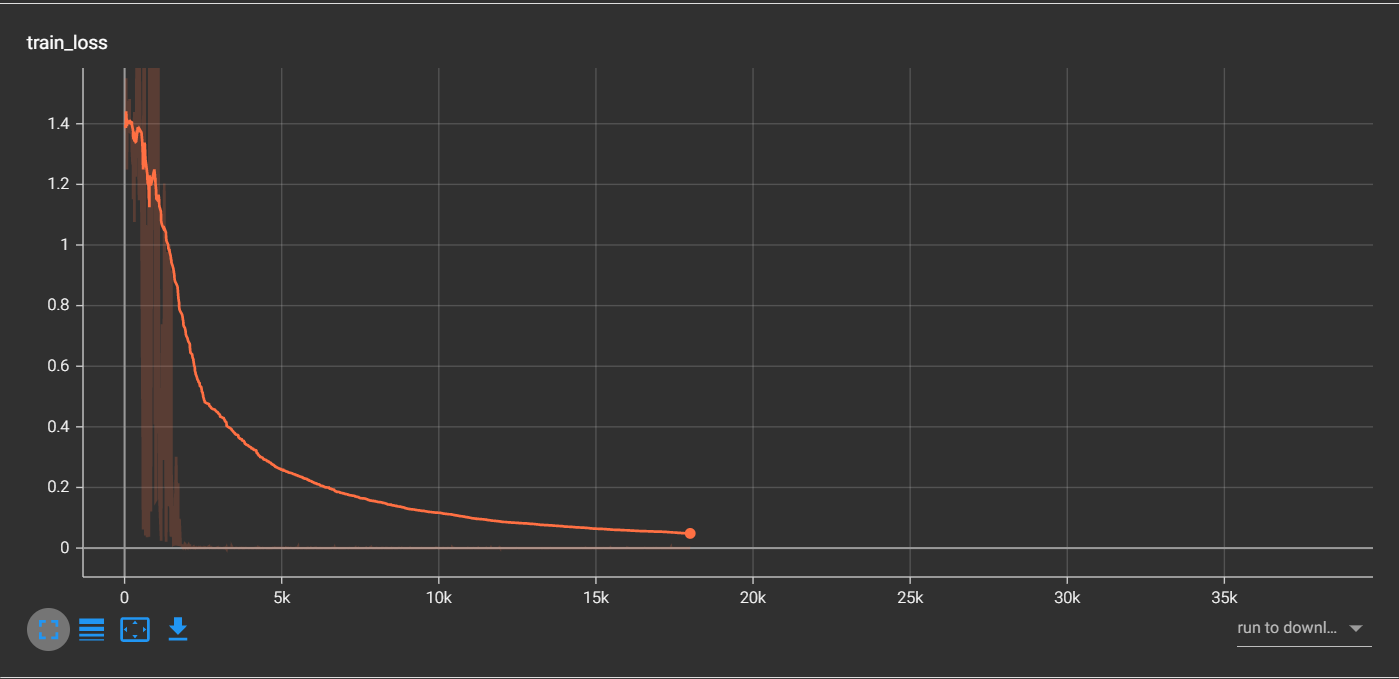
\includegraphics[width=2in]{figure/Train_loss.png}
				\caption{训练损失}
			\end{minipage}
		}
		\subfigure{
			\begin{minipage}[t]{0.4\linewidth}
				\centering
				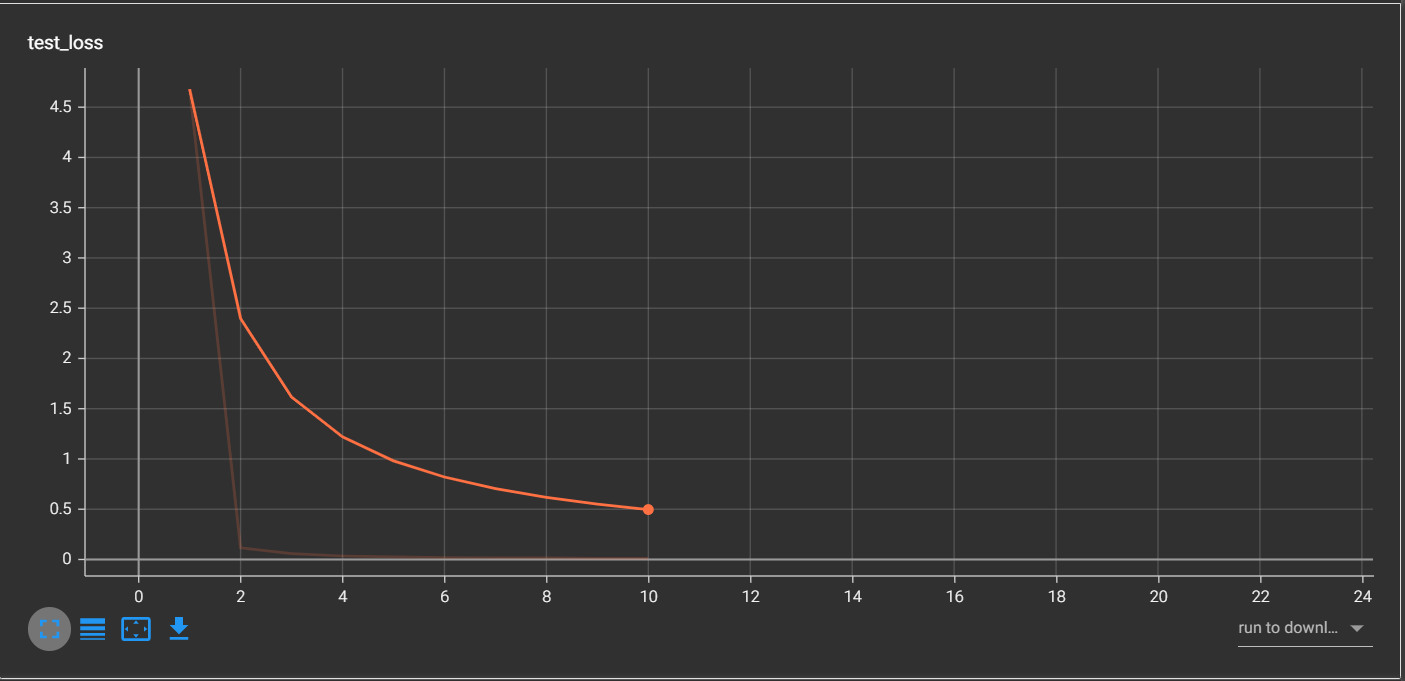
\includegraphics[width=2in]{figure/Test_loss.png}
				\caption{验证损失}
			\end{minipage}
		}
	\end{figure}

	可以看出损失函数最终收敛,同时,在运行面板上导出的数据也表明训练的结果非常好。第18000次迭代的训练损失值为7.27174e-06,第十轮的验证损失为0.01166687。
	
	\subsubsection{分类测试}
	
	编写测试代码。
	
	\begin{lstlisting}
	from PIL import Image
	from torchvision import transforms
	import Net_V2
	import torch
		
	net_test = Net_V2.Net()
	net_test.load_state_dict(torch.load(r'path'))
		
	img = Image.open(r'path')
	transform = transforms.ToTensor()
	img = transform(img)
	img = torch.reshape(img, [-1, 1, 128, 128])
	outs = net_test(img)
	out_index = outs.argmax(1)
	if out_index == 0:
		print("故障类别为1")
	elif out_index == 1:
		print("故障类别为4")
	elif out_index == 2:
		print("故障类别为7")
	elif out_index == 3:
		print("故障类别为8")
	else:
		print("无法判断")
	\end{lstlisting}
	
	这里的关键代码在1行中的-1,即Tensor变量中的批次值让计算机自动选取。
	
	修改img的图像路径,运行程序,发现取得非常好的分类效果。
	
	\begin{figure}[ht]
		\centering
		\subfigure{
			\begin{minipage}[t]{1\linewidth}
				\centering
				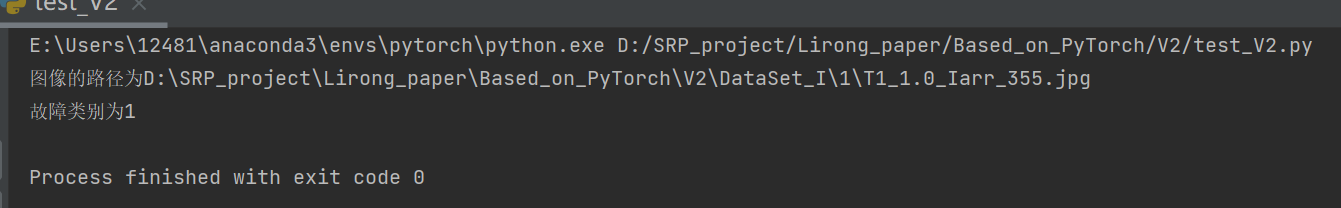
\includegraphics[width=6in]{figure/7.png}
				\caption{故障1测试}
			\end{minipage}
		}
	
		\subfigure{
			\begin{minipage}[t]{1\linewidth}
				\centering
				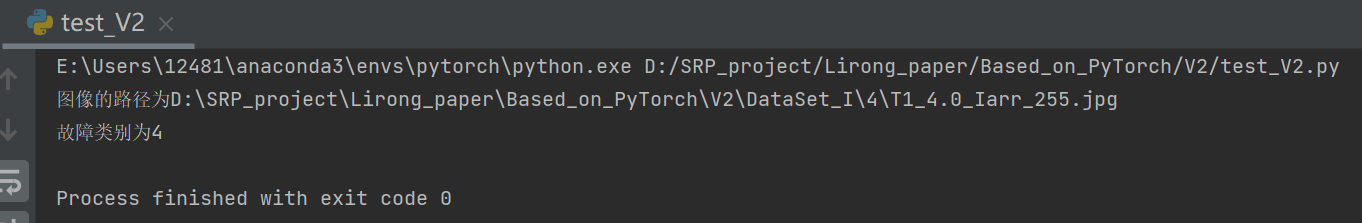
\includegraphics[width=6in]{figure/8.png}
				\caption{故障4测试}
			\end{minipage}
		}
		
		\subfigure{
			\begin{minipage}[t]{1\linewidth}
				\centering
				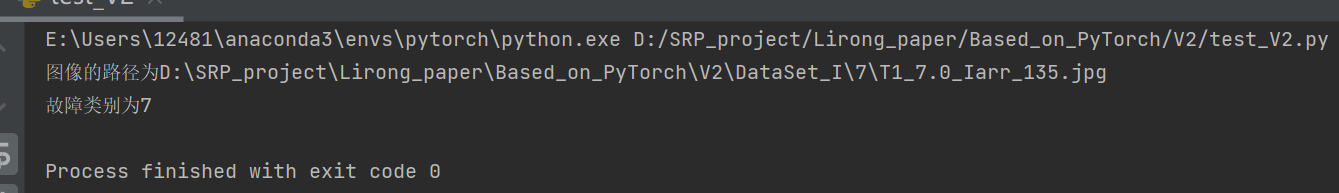
\includegraphics[width=6in]{figure/9.png}
				\caption{故障7测试}
			\end{minipage}
		}
	
		\subfigure{
			\begin{minipage}[t]{1\linewidth}
				\centering
				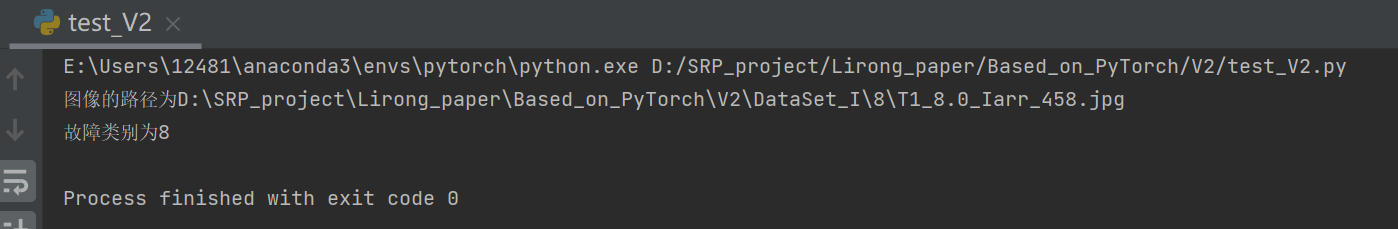
\includegraphics[width=6in]{figure/10.png}
				\caption{故障8测试}
			\end{minipage}
		}
		
	\end{figure}

	至此,达到了最初的目的,实现了对故障类型的分类处理。
	
	整个流程看下来,存在一些需要改进的地方,比如模型结构上,第一层池化的池化核大小可以改小一些;数据集打标签的部分需要完善程序。下一周计划对这些做出改进,同时在现有的基础上实现对故障定位的功能。
	
\end{document}